% !TEX root = 99_main.tex


\subsection{Overview of feedback data}



%Figure \ref{fig:hourPlot} details a simple heat-map where the user comfort feedback is mapped to the hour of the day. Users appear to be comfortable on average [INSERT NUMEBR HERE] \% of the time, and there are no statistically significant trends during working hours (9:00 - 17:00). Variations in user comfort feedback during the day can be used to infer an issue within the building.

%It is interesting to note that there is on average [INSERT NUMBER HERE] times more responses in the hours of 9:00, 11:00, 13:00, 15:00, and 17:00 when the occupant is buzzed and forced to give feedback. Nevertheless there are still significant amounts of responses made outside these times through the motivation of the participants themselves. Figure \ref{fig:responseRate} details the daily responses from the participants, and no observable decrease in responses can be made. Dips in responses naturally occur during the weekend. 


\begin{figure}
\begin{center}
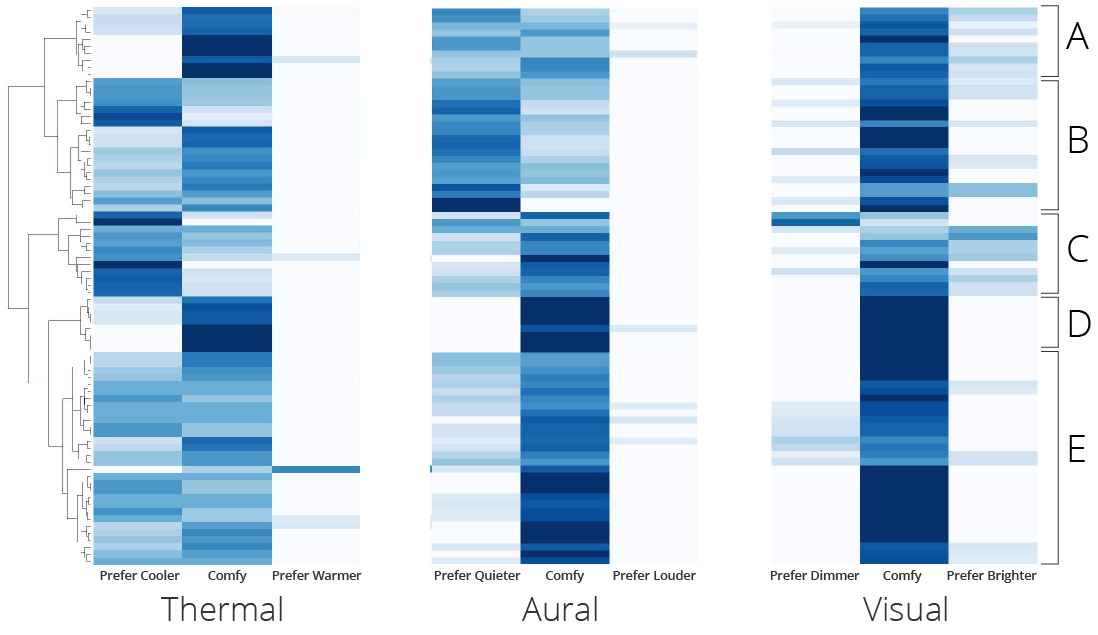
\includegraphics[width=\textwidth, trim= 0cm 0cm 0cm 0cm,clip]{Fig3.jpg}
\caption{Overview of Feedback Data (a) Split between outdoor vs. indoor feedback data (b) Distribution of votes between temperature, light and noise variables.}
\label{fig:feedbackdata}
\end{center}
\end{figure}


\subsection{Influence of environmental profiles of spaces}
\label{ch:userResults}

%Individual user feedback can be clustered using un-supervised learning techniques. In this example, we use a hierarchal k-means clustering based on euclidean distance using the Nearest-Point-Algorithm. The results, shown in Figure \ref{fig:clustering}, show four distinct clusters of users. 
%Users that are comfortable 100\% of the time, users that are comfortable 60-80 \% of the time, those that are comfortable 50\% of the time and generally would prefer it cooler, those that are comfortable 50\% of the time and would prefer it both warmer and cooler. 
%Understanding and defining these differences in user preferences can be used to recommend spaces that may better suit the needs of the occupant. For example, User 5 and User 10 can be recommended working spaces that are on average cooler. User 13 on the other hand appears to have a broad comfort spectrum. 

%It is importat to note that the data is not representative of a single space. As shown in Figure \ref{fig:map}, responses were made throughout Singapore. GPS data can support in localising responses to individual buildings, but also comes with issues which will be discussed in Section \ref{ch:localisation}.


%It is important to note here that the data is not entirely representative of a single building space, as the user may have given feedback while having lunch outside. There are even feedback results made outside of working hours as seen in \ref{fig:hourPlot} \ref{fig:responseRate}. Conclusions such as "Building Zone A was comfortable 80\% of the time" can therefore not be made. This will be further discussed in Section \ref{ch:discussion}.

\subsection{Influence of occupant comfort personality}

%It is widely known that heart-rate influences metabolic activity, and therefore an occupants comfort preference. Figure \ref{fig:heartHist} details the number of responses for each thermal response based on the heart rate. [INSERT NUMBER HERE ] \% of "Prefer Cooler" responses occurred during higher metabolic activity when the heart rate was greater than 100 beats per minute. If we filter out these responses,and apply the same algorithms detailed in Section \ref{ch:userResults}, we see a slightly different response and clustering pattern, as shown in Figure \ref{fig:lowHeartUsers}. 

\begin{figure}
\begin{center}
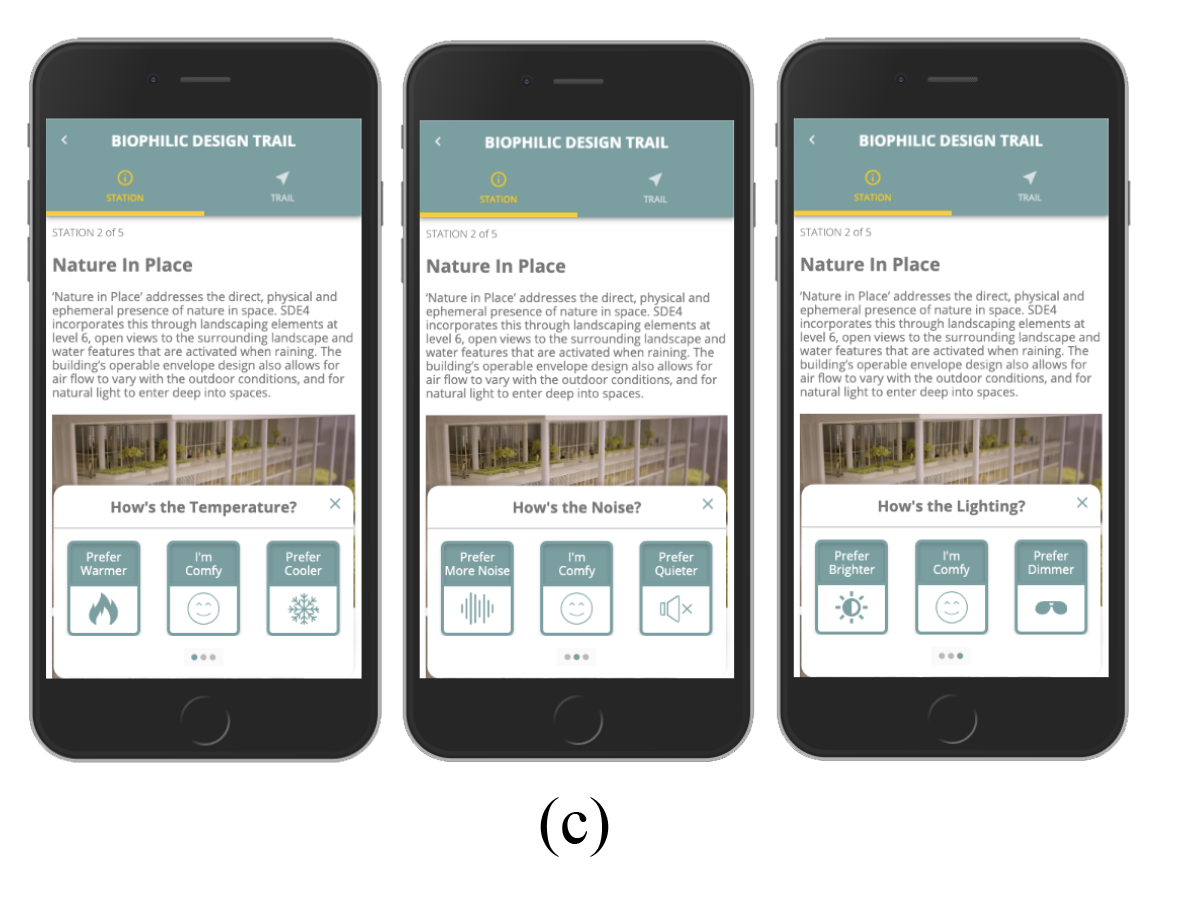
\includegraphics[width=\textwidth, trim= 0cm 0cm 0cm 0cm,clip]{Fig4.jpg}
\caption{Clustering (a) Clustering space type based on user feedback (b) Clustering users based on comfort preferences.}
\label{fig:Clustering}
\end{center}
\end{figure}




\subsection{Correlations between environemntal attributes in different types of spaces}

%Combining the cozie watch face, with the "strap-pack", an environmental sensor addition to the watch face opens another dimension of analysis. User responses are mapped to the environmental condition at which they are exposed to, which can provide a high quality labeled data set for training data driven models. Figure \ref{fig:tempHist} detail the temperatures at which responses were mapped. Note that the temperature of the strap sensor is on average 0.8 $^\circ$C warmer than the surrounding environment due to the influence of body temperature. 

\begin{figure}
\begin{center}
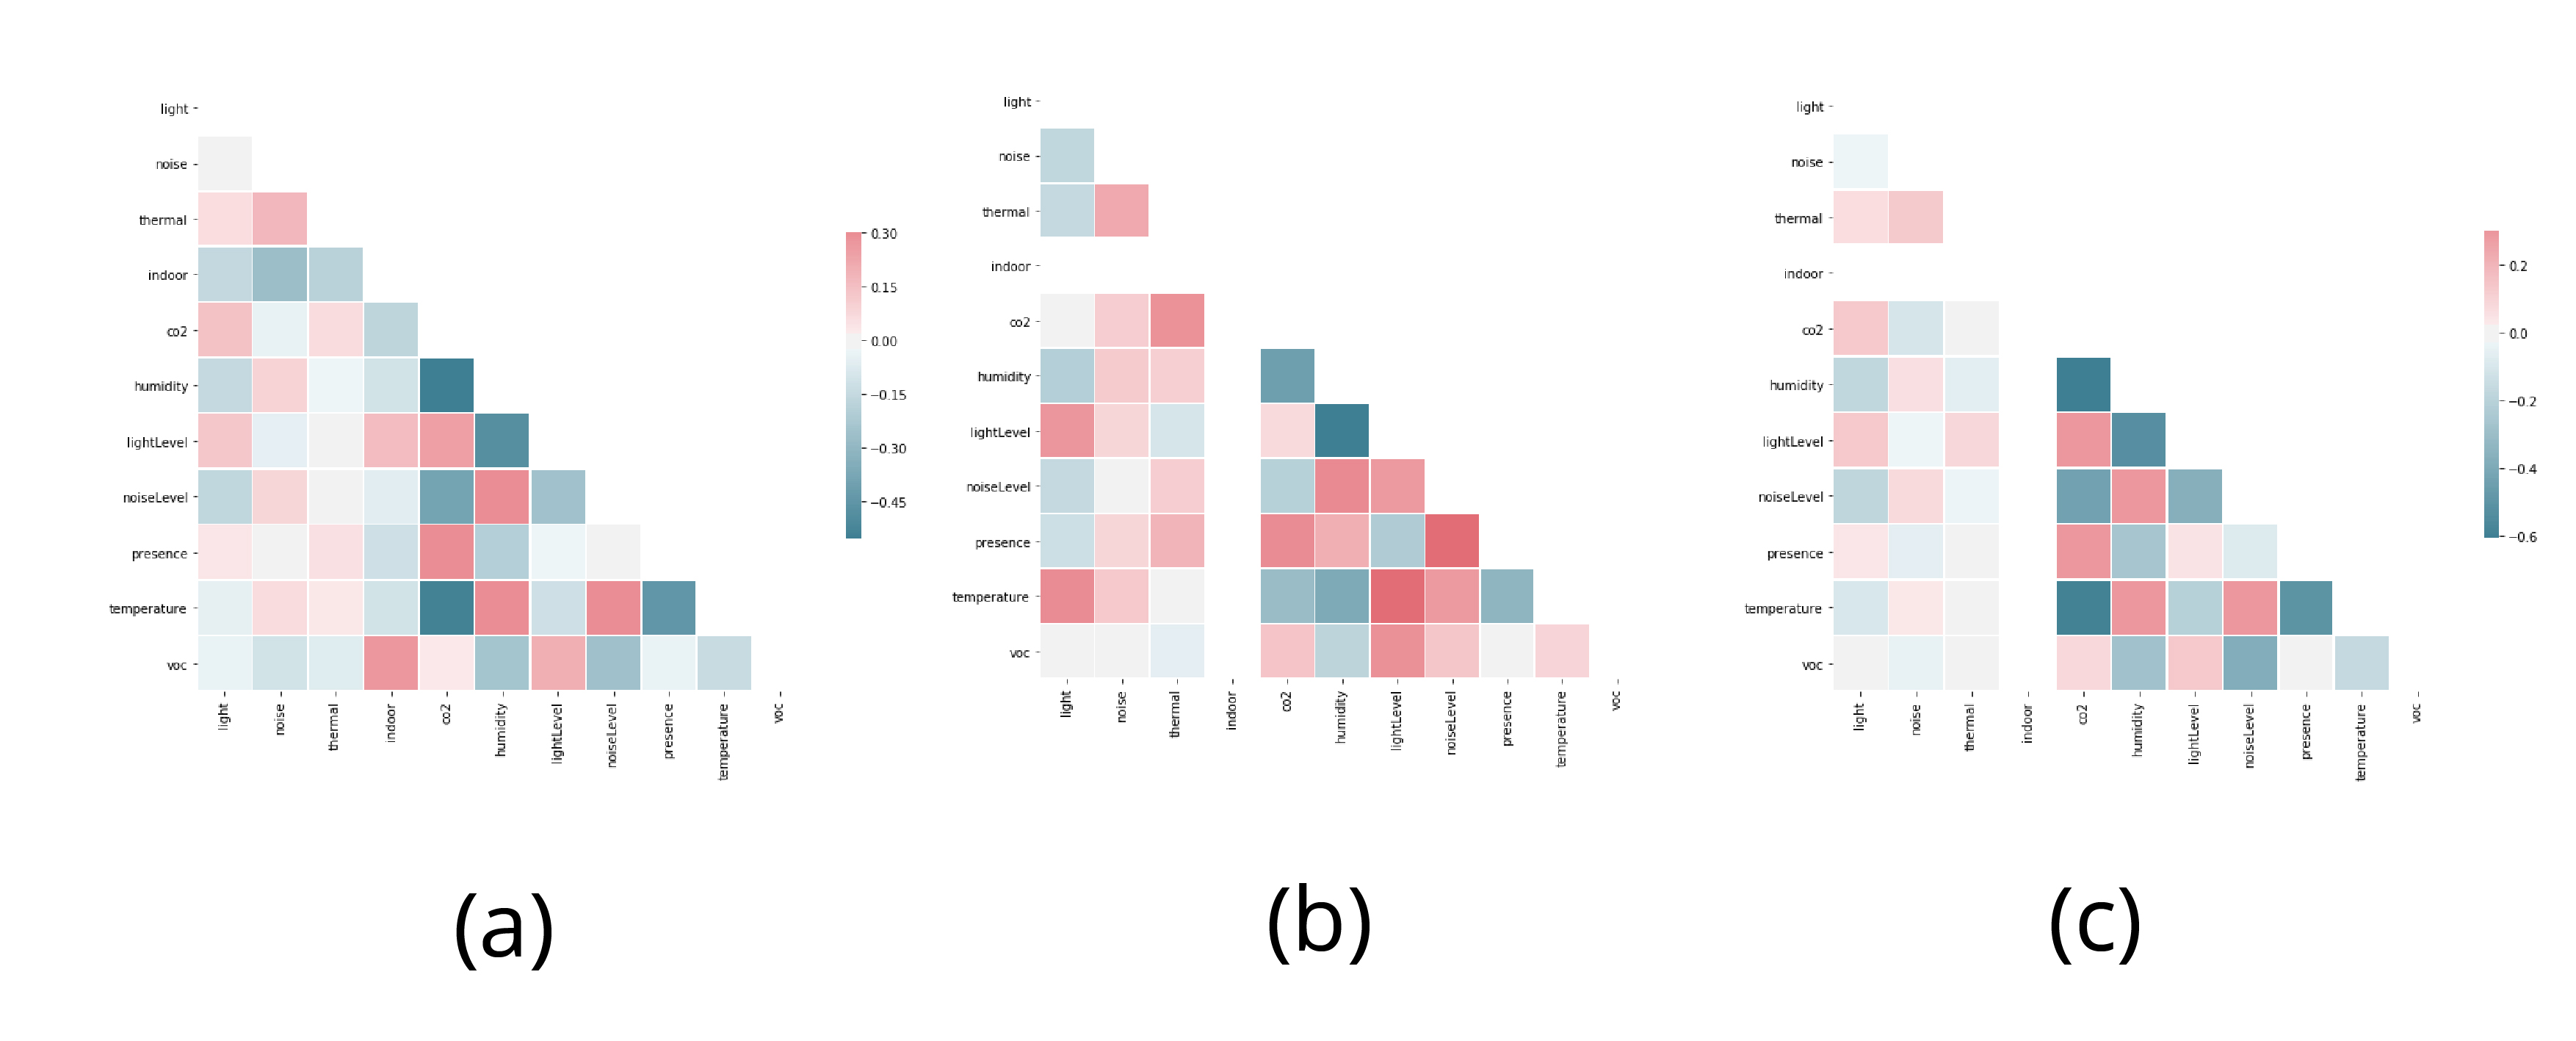
\includegraphics[width=\textwidth, trim= 0cm 0cm 0cm 0cm,clip]{Fig5.jpg}
\caption{Correlations (a) Overall (b) Indoor spaces, (c) Outdoor spaces.}
\label{fig:Clustering}
\end{center}
\end{figure}



% convert time to bars
% one heart rate filter showing. Groups of similar behaving people. Group 1-4. What are the coincidental ranges of data belonging to these groups. 